% -*- TeX:SI -*-
% slovene sub-mode for spell check
%%%%%%%%%%%%%%%%%%%%%%%%%%%%%%%%%%%%%%%%%%%%%%%%%%%%%%%%%%%%%%%%%%%%%%%%%%%%%%%%%%%%%%%%%%%%%%%%%%%%%%%%%%%%%%%%%%%%%%%%
% LaTeX predloga za zaključna dela
% Univerza v Ljubljani, Fakulteta za elektrotehniko
% Zbral in uredil: Roman Kamnik, junij 2013
% Dopolnil: Sebastjan Šlajpah (2013), Sašo Tomažič (2013), Peter Miklavčič (2019)
%%%%%%%%%%%%%%%%%%%%%%%%%%%%%%%%%%%%%%%%%%%%%%%%%%%%%%%%%%%%%%%%%%%%%%%%%%%%%%%%%%%%%%%%%%%%%%%%%%%%%%%%%%%%%%%%%%%%%%%%
\documentclass[a4paper,twoside,openright,12pt,slovene]{book}
\usepackage[pdftex]{UNI-LJ-FE-Diploma} % stil zaključnega dela UL FE
\usepackage[utf8]{inputenc} % predloga uporablja standardno kodiranje Unicode UTF-8, ki podpira šumnike
\usepackage[greek,english,slovene]{babel} % seznam uporabljenih jezikov (zadnji na seznamu je primarni)

% PDF/A %%%%%%%%%%%%%%%%%%%%%%%%%%%%%%%%%%%%%%%%%%%%%%%%%%%%%%%%%%%%%%%%%%%%%%%%%%%%%%%%%%%%%%%%%%%%%%%%%%%%%%%%%%%%%%%%
% Več o PDF/A v LaTeX-u: https://www.mathstat.dal.ca/~selinger/pdfa/
\usepackage{filecontents}
\begin{filecontents*}{\jobname.xmpdata}
    \Title{Navodila in predloga za izdelavo zaključnega dela} % Mora biti enak kot je v prijavi teme!
    \Author{Ime in priimek avtorja} % Mora biti enak kot na naslovnici!
\end{filecontents*}
\usepackage[a-1b]{pdfx}
%%%%%%%%%%%%%%%%%%%%%%%%%%%%%%%%%%%%%%%%%%%%%%%%%%%%%%%%%%%%%%%%%%%%%%%%%%%%%%%%%%%%%%%%%%%%%%%%%%%%%%%%%%%%%%%%%%%%%%%%

% LaTeX PAKETI %%%%%%%%%%%%%%%%%%%%%%%%%%%%%%%%%%%%%%%%%%%%%%%%%%%%%%%%%%%%%%%%%%%%%%%%%%%%%%%%%%%%%%%%%%%%%%%%%%%%%%%%%
% Kompakten pregled LaTeX ukazov je dostopen na https://en.wikibooks.org/wiki/Category:Book:LaTeX
% Navodila posameznih uporabljenih paketov so dostopna na https://www.ctan.org

% Dodatni simboli
\usepackage{textcomp}                               % dodatni simboli (kot npr. €)
\usepackage{gensymb}                                % dodatni simboli \de­gree, \cel­sius, \pert­hou­sand, \mi­cro, \ohm
\newcommand{\uppi}{\textrm{\greektext p\latintext}} % velika grška črka P z \uppi, alternativa simbolu \Pi

% Osnovno oblikovanje
\hypersetup{unicode,hidelinks,breaklinks,hyperindex} % dodatne možnosti hiperpovezav
\usepackage[normalem]{ulem}                          % podčrtavanje in prečrtavanje teksta
\usepackage{float}                                   % dodatne možnosti oblikovanja objektov
\usepackage{enumitem}                                % dodatne možnosti oblikovanja seznamov

% Dodatno oblikovanje
%\zamaknirobsodihstrani{0mm} % dodatna prilagoditev levega roba sodih strani za dvostranski tisk
%\usepackage{dcolumn}        % poravnava po decimalnih mestih v tabelah
%\usepackage{longtable}      % večstranske tabele
%\usepackage{caption}        % dodatne možnosti označevanja objektov
%\usepackage{rotating}       % vretenje objektov, strani, ipd.

% Matematična orodja
\usepackage{mathtools} % http://mirrors.ctan.org/macros/LaTeX/contrib/mathtools/mathtools.pdf
\usepackage{bm}        % ukaz za odebeljeni tisk \bm v matematičnih okoljih
%\usepackage{cancel}   % ukaz za prečrtavanje \cancel v matematičnih okoljih

% Grafična orodja
\usepackage{graphicx}                 % vključevanje bitnih slik z ukazom \includegraphics
\usepackage{grffile}                  % podpora presledkom pri ukazu \includegraphics
%\usepackage{tikz}                    % paket TikZ za risanje (npr. blokovnih shem, diagramov poteka, itd.)
%\usetikzlibrary{calc,shapes,arrows}  % dodatne možnosti paketa TikZ
%\usepackage{tikzscale}               % skaliranje risb
%\usepackage[smartlabels]{circuitikz} % risanje shem vezij
%\usepackage{pgfplots}                % paket PGFPlots za risanje grafov, tudi iz CSV in podobnih datotek
%\usepgfplotslibrary{polar,external}  % dodatne možnosti paketa PGFPlots
%\usepackage{tikz-3dplot}             % 3D risanje
% Primeri: http://texample.net , http://pgfplots.net/tikz/examples , http://pgfplots.sourceforge.net/gallery.html

% Vključevanje datotek
\usepackage{pdfpages} % vključevanje PDF datotek z ukazom \includegraphics
\usepackage{epstopdf} % vključevanje EPS datotek z ukazom \includegraphics
\usepackage{listings} % orodja za izpisovanje programske kode
\lstset{              % nastavitve orodja za izpisovanje programske kode
    basicstyle=\ttfamily\footnotesize,
    breaklines=true,
    numbers=left,
    numberstyle=\scriptsize,
    keywordstyle=\color{blue},
    commentstyle=\color{unilj},
    stringstyle=\color{olive},
}
%%%%%%%%%%%%%%%%%%%%%%%%%%%%%%%%%%%%%%%%%%%%%%%%%%%%%%%%%%%%%%%%%%%%%%%%%%%%%%%%%%%%%%%%%%%%%%%%%%%%%%%%%%%%%%%%%%%%%%%%

% DEKLARACIJE %%%%%%%%%%%%%%%%%%%%%%%%%%%%%%%%%%%%%%%%%%%%%%%%%%%%%%%%%%%%%%%%%%%%%%%%%%%%%%%%%%%%%%%%%%%%%%%%%%%%%%%%%%
\naslov{Navodila in predloga za izdelavo zaključnega dela} % Mora biti enak kot je v prijavi teme!
\avtor{Ime in priimek avtorja} % Mora se ujemati s \Title pri metapodatkih PDF/A!
\mentor{Naziv ter ime in priimek mentorja}
%\somentor{Naziv, ime in priimek somentorja}
\date{Ljubljana, \the\year}
\univerza{Univerza v Ljubljani}
\definecolor{unilj}{cmyk}{0.00, 0.94, 0.94, 0.06} % barva Univerze v Ljubljani

% Potrebno je paziti, da je izbrana prava kombinacija tipa dela in sodelujočih fakultet glede na študijski program!
\delo{Diplomsko delo\\~\\Univerzitetni študijski program prve stopnje Elektrotehnika}
%\delo{Diplomsko delo\\~\\Univerzitetni študijski program prve stopnje Multimedija}
%\delo{Diplomsko delo\\~\\Visokošolski strokovni študijski program\\prve stopnje Aplikativna elektrotehnika}
%\delo{Diplomsko delo\\~\\Visokošolski strokovni študijski program\\prve stopnje Multimedijske komunikacije}
%\delo{Magistrsko delo\\~\\Magistrski študijski program druge stopnje Elektrotehnika}
%\delo{Magistrsko delo\\~\\Magistrski študijski program druge stopnje Uporabna statistika}
\fakulteta{Fakulteta za elektrotehniko}
%\fakulteta{Fakulteta za elektrotehniko,\\Fakulteta za računalništvo in informatiko} % Za program Multimedija
%\fakulteta{Fakulteta za elektrotehniko, Biotehniška fakulteta,\\Ekonomska fakulteta, Fakulteta za družbene vede,\\Fakulteta za matematiko in fiziko, Fakulteta za\\računalništvo in informatiko, Medicinska fakulteta} % Za program Uporabna statistika
%%%%%%%%%%%%%%%%%%%%%%%%%%%%%%%%%%%%%%%%%%%%%%%%%%%%%%%%%%%%%%%%%%%%%%%%%%%%%%%%%%%%%%%%%%%%%%%%%%%%%%%%%%%%%%%%%%%%%%%%

% DOKUMENT %%%%%%%%%%%%%%%%%%%%%%%%%%%%%%%%%%%%%%%%%%%%%%%%%%%%%%%%%%%%%%%%%%%%%%%%%%%%%%%%%%%%%%%%%%%%%%%%%%%%%%%%%%%%%
\begin{document}
\frontmatter

\selectlanguage{slovene}

%******************************* NASLOVNICA ************************************
\maketitle

%******************************* ZAHVALA ***************************************
\zahvala
V zahvali se kandidat lahko zahvali mentorju in poimensko tudi vsem sodelavcem in prijateljem, ki so pomagali in prispevali pri delu v laboratoriju, na računalniku, v delavnici, pri tehnični izdelavi dela ali drugje.

%******************************* POVZETEK IN KLJUČNE BESEDE ********************
\povzetek
V tem dokumentu so predstavljena navodila za izdelavo zaključnega dela na Fakulteti za elektrotehniko v Ljubljani. Zaključno delo predstavlja diplomsko delo na prvi in magistrsko delo na drugi stopnji izobraževalnega programa.

V povzetku v slovenščini in v angleščini kandidat navede glavne rezultate dela, zato naj povzetek seznani bralca z jedrom dela na način, ki je običajen za pisanje krajših člankov ali referatov. Obseg povzetka je za Repozitorij Univerze v Ljubljani omejen na 20.000 znakov.

Povzetek se prične z opisom in definicijo problema. Nadaljuje se z opisom uporabljenih metod in postopkov, ki so privedli do rešitve. Na koncu so opisani rezultati dela in glavni zaključki, ki iz rezultatov izhajajo.

Za povzetkom se na isti strani navede še ključne besede.

\kljucnebesede
beseda1, beseda2, ...

\selectlanguage{english}

%******************************* ABSTRACT AND KEYWORDS *************************

\abstract
The thesis addresses...

\keywords
word1, word2, ...

\selectlanguage{slovene}

%******************************* KAZALO ****************************************
\tableofcontents

%******************************* SEZNAM SLIK, SEZNAM TABEL *********************
\seznamslik
\seznamtabel

%******************************* SEZNAM SIMBOLOV *******************************
\seznamsimbolov
V pričujočem zaključnem delu so uporabljene naslednje veličine in simboli:

\begin{center}
    \begin{tabular}{*{4}{l}} \hline
        \multicolumn{2}{c}{\bf{Veličina / oznaka}}           & \multicolumn{2}{c}{\bf{Enota}} \\ \hline
        Ime                & Simbol                          & Ime      & Simbol              \\ \hline
        čas                & $t$                             & sekunda  & s                   \\
        frekvenca          & $f$                             & Hertz    & Hz                  \\
        tlak               & $p$                             & Pascal   & Pa                  \\
        sila vzgona        & $\textbf{\textit{F}}_\text{vz}$ & Newton   & N                   \\
        gostota            & $\rho$                          & -        & kg/m$^3$            \\
        masa               & $m$                             & kilogram & kg                  \\
        vhodna napestost   & $U_\text{vh}$                   & volt     & V                   \\
        Jacobijeva matrika & $\mathbf{J}$                    & -        & -                   \\ \hline
    \end{tabular}
\end{center}

Pri čimer so vektorji in matrike zapisani s poudarjeno pisavo. Natančnejši pomen simbolov ter njihovih indeksov je razviden iz ustreznih slik ali pa je pojasnjen v spremljajočem besedilu, kjer je simbol uporabljen.

\mainmatter

%******************************* UVOD ******************************************
\chapter{Uvod} \label{uvod}

Uvod v zaključno delo ima namen, da uvede bralca v tematiko zaključnega dela. V njem kandidat razčleni zahteve in cilje zaključnega dela, po literaturi povzame znane rešitve in oceni njihov pomen za zaključno delo. Sklicevanje na literaturo se v besedilu označi s številko v oglatem oklepaju, ki jo ima ta v seznamu uporabljenih virov, in po potrebi navede strani, npr. \cite{miklavcic2010objavljanje} ali \cite[stran 520-534]{juznic1992diplomska}.

%******************************* POGLAVJA **************************************

\chapter{Izbira teme zaključnega dela} \label{izbira_teme}

Zaključno delo je zasnovano na znanju, sposobnostih in veščinah, ki jih je študent pridobil med študijem. V zaključnem delu študent samostojno obdela strokovni problem, pri katerem izkaže svojo ustvarjalno sposobnost za razvojno in raziskovalno delo, predvsem pa zmožnost, da pridobljeno znanje uspešno in celovito uporabi pri izdelavi svojega dela. Delo na zaključni temi ni in ne more biti le pridobivanje novega znanja. Z njim študent dokaže sposobnost analiziranja, kritičnega ocenjevanja, uporabe literature, samostojnega sklepanja in presoje in s tem usposobljenost za strokovno delo in reševanje strokovnih problemov. Zaključno delo je lahko tudi rezultat dela več študentov, pri čimer mora biti jasno razviden prispevek posameznega študenta.

Fakultetni učitelji imajo pravico in dolžnost predlagati okvirne teme zaključnega dela. Pri tem lahko po svoji presoji vključijo tudi somentorja, kadar zajame tema širše oziroma interdisciplinarno področje. Študent izbere temo zaključnega dela praviloma s tistih elektrotehniških področij, ki so ključna za oblikovanje profila določene smeri študija. Pravica študenta pa je, da samostojno izbira temo, kar lahko stori na dva načina:
\begin{enumerate}[noitemsep]
    \item lahko si izbere katero izmed tem, ki jih fakulteta oziroma posamezni fakultetni učitelji razpisujejo za tekoče študijsko leto,
    \item lahko si najprej izbere mentorja iz vrst habilitiranih učiteljev za določeno strokovno področje in se z njim dogovori za temo zaključnega dela. V tem primeru lahko ta zajema tudi problematiko neke gospodarske organizacije, štipenditorja in podobno.
\end{enumerate}

Pri izbiri teme zaključnega dela je treba upoštevati aktualnost problema, materialne možnosti in potreben čas za izdelavo dela. Z mentorjem je potrebno uskladiti pričakovan obseg dela. Postopek za prijavo teme zaključnega dela je opisan na spletnih straneh Študentske pisarne FE: \url{http://www.fe.uni-lj.si/izobrazevanje/studentska\_pisarna/}. Urejeno zaključno delo študent izdela in odda v predvidenem času glede na posamezen študijski program. Podrobnosti ureja Izpitni pravilnik UL FE.

\chapter{Opravljanje zaključnega dela} \label{opravljanje_naloge}

\begin{itemize}

\item Zaključno delo je kandidatovo prvo večje samostojno strokovno delo, zato naj se ga loti sistematično in z vso resnostjo.

\item Zaključno delo lahko kandidat opravi na fakulteti, v gospodarski družbi, pri štipenditorju ali drugje, o čimer se dogovori z mentorjem.

\item Pri opravljanju zaključnega dela mora kandidat strogo upoštevati pravila o varstvu pri delu, hišni red in ostala pravila fakultete ali gospodarske organizacije, v kateri opravlja zaključno delo.

\item Za uspešno delo je zelo pomembno dobro sodelovanje kandidata z mentorjem, zato se kandidat redno in po dogovoru posvetuje s svojim mentorjem ter ga sproti obvešča o opravljenem delu. Morebitno sodelovanje z drugimi sodelavci na fakulteti ali zunaj nje poteka v soglasju z mentorjem.

\item Za kvalitetno zaključno delo je pomembna tudi uporaba vseh razpoložljivih domačih in tujih strokovnih ter znanstvenih virov.

\item Če pride med opravljanjem zaključnega dela do nesoglasja med kandidatom in mentorjem (ali somentorjem), ki onemogoči ustvarjalno sodelovanje, ima kandidat na podlagi sklepa Študijske komisije pravico do zamenjave mentorja (ali somentorja). Za to je potrebno z navedbo razlogov pisno zaprositi Študijsko komisijo FE, ki na podlagi sklepa odobri zamenjavo in določi novega mentorja (ali somentorja). Kandidat ima pravico do zamenjave mentorja (ali somentorja) le enkrat. Tudi mentor (ali somentor) lahko po enakem postopku odkloni mentorstvo (oziroma somentorstvo).

\end{itemize}

\chapter{Pisanje zaključnega dela} \label{pisanje_dela}

\begin{itemize}

\item Pri pisanju zaključnega dela izkazuje kandidat poleg strokovne usposobljenosti tudi splošno razgledanost.

\item Zaključno delo je praviloma napisano v slovenskem jeziku in mora biti jezikovno neoporečno. Kandidatu se dovoli pisanje zaključnega dela v tujem jeziku na osnovi utemeljene prošnje. Priporočamo, da pisni izdelek pred oddajo pregleda lektor.

\item Obseg (dolžina) zaključnega dela se določi v dogovoru z mentorjem.

\item Kadar za določen strokovni termin ni splošno sprejetega domačega izraza, se prvič, ko se slovenski izraz pojavi, v oklepaju navede originalni izraz, povzet iz uporabljene literature, npr. impedančno vodenje (ang. impedance control).

\item Plagiatorstvo, ne glede na obliko in način predstavljanja tujega avtorskega dela kot svojega, je v nasprotju z akademsko etiko in pomeni hujšo kršitev pravil ter predpisov, ki to področje urejajo in je podlaga za odvzem strokovnega naslova.

\end{itemize}

\section{Oblika zaključnega dela} \label{oblika_dela}

Besedilo mora biti napisano na belem papirju formata A4. Tisk je praviloma obojestranski. Kandidat potrebuje tri izvode zaključnega dela (zase, za mentorja in knjižnico fakultete).

Razmik med vrsticami naj bo 1,2, okvirna postavitev besedila pa naj bo 20 mm od zunanjega in zgornjega roba (nad pagino vivo, če je ta uporabljena) ter 30 mm od notranjega in spodnjega roba.

Celoten izdelek naj bo vezan v trdo platno ali drug ustrezen material poljubne barve. Na hrbtni strani oz. hrbtišču (ne na zadnji platnici!) vezanega dela naj bosta napisana ime in priimek kandidata ter vrsta zaključega dela (``Magistrsko delo'' ali ``Diplomsko delo'').

\section{Zgradba zaključnega dela} \label{zgradba_dela}

\begin{enumerate}

\item Platnica naj vsebuje (sredinsko poravnano):
\begin{itemize}[noitemsep]
    \item naziv univerze in fakultet(e) z večjimi črkami, oddaljen ca. 30 mm od zgornjega roba,
    \item ime in priimek kandidata,
    \item naslov zaključnega dela (enak, kot v originalu izdane teme!), napisan z večjimi črkami,
    \item oznako vrste zaključnega dela (npr. Diplomsko ali Magistrsko delo),
    \item naziv študijskega programa,
    \item napis ``Ljubljana, letnica'', oddaljen ca. 30 mm od spodnjega roba.
\end{itemize}
Platnica je enaka naslovni (prvi) strani, le da ne vsebuje navedbe mentorjev. Tudi pri zaključnih delih, napisanih v tujem jeziku, mora biti platnica v slovenskem jeziku.

Znotraj platnic si po naslednjem vrstnem redu najprej sledijo uvodne strani:

\item Naslovna (prva) stran je enaka platnici, le da vsebuje še navedbo mentorja. Enotno oblikovana naslovna stran, ki je namenjena tiskanim izvodom dela, je po oddaji elektronske različice naloge na voljo v sistemu Studis. Iz te datoteke se izdela tudi platnica (brez navedb mentorjev). V primeru dela v tujem jeziku, je prva stran zaključnega dela v tujem jeziku, sledi pa ji še ena prva stran v slovenskem jeziku.

\item Originalne listine prijavljene teme zaključnega dela kandidat dvigne v študentski pisarni, preden odda izdelek v vezavo.

\item Izjava kandidata o avtorstvu, istovetnosti elektronske in tiskane verzije ter avtorskih pravicah. Tako kot naslovna (prva) stran, je tudi ta na voljo v sistemu Studis.

\item Morebitna zahvala, v kateri se kandidat lahko zahvali mentorju in poimensko tudi vsem sodelavcem in prijateljem, ki so pomagali in prispevali pri delu v laboratoriju, na računalniku, v delavnici, pri tehnični izdelavi dela ali drugje.

\item Morebitno posvetilo.

\item V povzetku v slovenščini in v enem izmed tujih jezikov, ki praviloma obsega največ eno stran, kandidat navede glavne rezultate dela, zato naj povzetek seznani bralca z jedrom dela na način, ki je običajen za pisanje krajših člankov ali referatov. Za posameznim povzetkom se na isti strani navede še ključne besede v ustreznem jeziku. V primeru tujejezičnega dela, mora povzetek zaključnega dela v slovenskem jeziku obsegati 3 do 5 strani (razširjen povzetek).

\item Kazalo, seznam slik, tabel in uporabljenih simbolov, ki morajo biti enotni v celotnem delu, ne glede na označevanje v uporabljenih virih.

\end{enumerate}

Uvodni del nima označb strani ali pa se uporabi male tiskane rimske številke (kot v pričujočem dokumentu). Glavni del zaključnega dela obsega:

\begin{itemize}

\item Uvod v zaključno delo ima namen, da uvede bralca v tematiko zaključnega dela. V njem kandidat razčleni zahteve in cilje zaključnega dela, po literaturi povzame znane rešitve in oceni njihov pomen za zaključno delo. Sklicevanje na literaturo se v besedilu označi s številko v oglatem oklepaju, ki jo ima ta v seznamu uporabljenih virov, in po potrebi navede strani, npr. [13, stran 520 - 534].

\item Glavni del, ki je smiselno razdeljen na več oštevilčenih poglavij ter podpoglavij (npr. pregled področja, teoretični del, praktični del, analizo rezultatov, ...), vsebuje sistematično opisano opravljeno delo, računske rezultate, opis merilnih vezav, merilnih rezultatov in oceno točnosti rezultatov. Slog mora biti kratek, jedrnat, informativen, strokovno eksakten in korekten. Zmotno je mnenje, da je zajetno zaključno delo nujno tudi znak kandidatovega obsežnega dela. V zaključnem delu kandidat ne prevaja ali prepisuje del in daljših razlag drugih avtorjev. Navaja le njihove rezultate, navede izhodiščne predpostavke in področje veljavnosti.

\item Sklepne ugotovitve naj prikažejo oceno opravljenega dela ter povzamejo težave, na katere je kandidat naletel. Kot rezultat dela so lahko navedene tudi ideje, nastale med delom, ki bi lahko bile predmet novih raziskav.

\item Vire se navaja v posebnem seznamu v vrstnem redu, kot so prvič omenjeni v besedilu. Vselej se omejuje samo na pomembne vire in dolg seznam še zdaleč ni dokaz, da kandidat tak pregled nad literaturo tudi resnično ima. Podrobna navodila za navajanje posameznih vrst dokumentov so podana v spletnem dokumentu \cite{oven2013}. Nekaj pogostih primerov navedkov:
\begin{itemize}[noitemsep]
    \item Primer stavka, ki citira knjigo \cite{juznic1992diplomska}.
    \item Primer stavka, ki citira članek \cite{kuscer1996}.
    \item Primer stavka, ki citira prispevek iz zbornika s konference \cite{ambrozic2012}.
    \item Primer stavka, ki citira vir s spletne strani \cite{bor2006}.
\end{itemize}

\item Morebitne priloge (daljše računalniške izpise, risbe, konstrukcijske načrte, registracijo merilnih rezultatov, daljša izvajanja in podobno) kandidat izdela kot posebno poglavje po glavnem delu naloge. Vsaka priloga mora biti naslovljena in oštevilčena. Primer: priloga \ref{prilogaA}.

\end{itemize}

\section{Vključitev vsebin} \label{primeri_vsebin}

Navajanje tehničnih podatkov v tehniških tekstih zahteva določeno obliko. V tem poglavju so prikazani najpogostejši primeri vključevanja vsebin. Nekaj koristnih napotkov se najde v spletnem dokumentu \cite{murovec2013}.

\subsection{Enačbe} \label{vnos_enacb}

Podrobna navodila za pisanje enačb in formul so podana posebej v podpoglavju \ref{vnos_enacb}. Oblika zapisa veličin in enačb naj bo usklajena s standardom SIST-V ISO/IEC Vodilo 99 \cite{standard_sist_v} in s serijo standardov SIST EN ISO 80000 \cite{standard_sist_80000}. V osnovi standard priporoča, da so simboli za spremenljive veličine zapisani v poševnem tisku (tudi če nastopajo kot indeks), simboli za nespremenljive veličine in enote pa pokončno. Formule in enačbe je potrebno oštevilčiti z zaporedno številko v oklepaju in se nanje tako tudi sklicevati. Vektorji in matrike so zapisani s poudarjeno pisavo. V tekstu je potrebno pojasniti pomen posameznih parametrov. Primer:

Enačba (\ref{eq1}) opisuje hitrost točke $\textbf{\textit{v}}$, ki se nahaja na telesu:
\begin{equation} \label{eq1}
    \textbf{\textit{v}} = \textbf{\textit{v}}_0 + \boldsymbol{\omega} \times \mathbf{r}
\end{equation}
pri čimer $\textbf{\textit{v}}_0$ predstavlja hitrost izhodišča koordinatnega sistema, $\boldsymbol{\omega}$ kotno hitrost, $\mathbf{r}$ pa vektor od izhodišča do točke.

Enačbo (\ref{eq1}) lahko zapišemo v sklopu enačb po komponentah kot:
\begin{eqnarray} % \nonumber prepreči številčenje posameznih enačb
    v_x  &=& v_{0x} + z \;\omega_y - y \;\omega_z \nonumber \\
    v_y  &=& v_{0y} + x \;\omega_z - z \;\omega_x  \\
    v_z  &=& v_{0z} + y \;\omega_x - x \;\omega_y \nonumber
\end{eqnarray}

Paket \texttt{mathtools} omogoča napreden zapis enačb, najrazličnejših matematičnih simbolov, oklepajev, funkcij, ipd. Svoboda pri zapisovanju zahteva sicer nekaj vaje, ampak so na srečo vse možnosti paketa dobro opisane v samih navodilih\footnote{Dostopno na: http://mirrors.ctan.org/macros/LaTeX/contrib/mathtools/mathtools.pdf}. Poleg navodil je na spletu možno najti ogromno različnih primerov, s katerimi si je možno pomagati. Spodnji primer prikazuje uporabo ukaza \texttt{\textbackslash underbrace} (v okolju \texttt{equation}).

Enačba (\ref{eq2}) predstavlja sprejeto moč $P_\textrm{RX}$ pri odbitemu signalu radarja na razdalji do tarče $R$ (in se imenuje \emph{radarska enačba}):
\begin{equation} \label{eq2}
        P_{\textrm{RX}} =
    \underbrace{
    \underbrace{
    \underbrace{
            \left( \frac{P_{\textrm{TX}} G_{\textrm{ANT}}}{1} \right)
    }_{\textrm{oddaja}}
        \cdot
    \underbrace{
            \left( \frac{1}{4\pi \textcolor{unilj}{R^2}} \right)
    }_{\textrm{razširjanje}}
    }_{\substack{\textrm{pretok moči}\\\textrm{napredujočih valov}}}
        \cdot
    \underbrace{
            \left( \frac{\vphantom{1} \sigma}{1} \right) % ukaz \vphantom poskrbi za ujemanje velikosti oklepajev (težava je v nizkem simbolu za sigmo)
    }_{\textrm{odboj}}
        \cdot
    \underbrace{
            \left( \frac{1}{4\pi \textcolor{unilj}{R^2}} \right)
    }_{\textrm{razširjanje}}
    }_{\textrm{pretok moči odbitih valov}}
        \cdot
    \underbrace{
            \left( \frac{A_{\textrm{ANT}}}{1} \right)
    }_{\textrm{sprejem}}
\end{equation}

\subsection{Slike} \label{vnos_slik}

Slik, ki skrajšujejo besedilo, ali pripomorejo k razumljivosti, naj bo čim več. Slike, grafi in fotografije morajo biti oštevilčeni in citirani v besedilu ter podnaslovljeni tako, da je razvidno, kaj predstavljajo. V besedilo so slike vstavljene približno tam, kjer se nanje sklicujemo. Morajo biti pregledne in jasno prikazati samo potrebno informacijo. Grafi na slikah morajo imeti pravilno označene osi, skalo, enote in legendo. Grafi so praviloma v enem izmed vektorskih zapisov, ki omogočajo višjo kvaliteto prikaza in tiska ter po nepotrebnem ne izgubljajo informacije. Napisi na sliki morajo biti v slovenskem jeziku. Primer je na sliki \ref{oblika_signalov_1}. Podrobnejša navodila o vključevanju vektorskih in bitnih slik v LaTeX dokumente vsebuje priloga \ref{prilogaB}.

\begin{figure}[h]
    \centering
    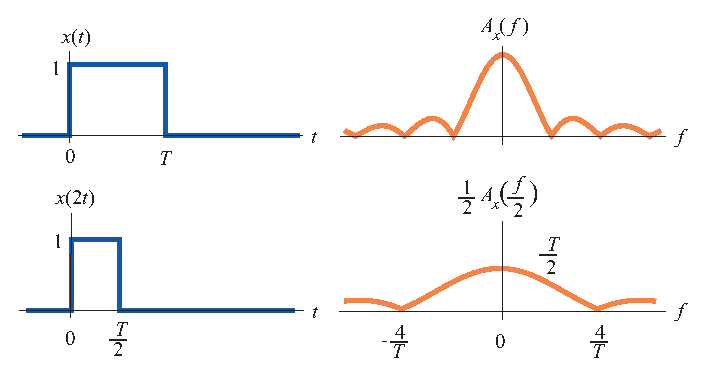
\includegraphics[width=0.75\columnwidth]{Slike/vektorska_slika_1.eps}
    \caption{\label{oblika_signalov_1} Primer vključitve slike.}
\end{figure}

\subsection{Programska koda}

Manjši deli programske kode so lahko navedeni in opisani v tekstu. Oblika teksta programske kode se loči od oblike ostalega teksta.
Primer:

Funkcija, ki omogoča prenos podatkov, je naslednja:

\lstset{language=C}
%\lstinputlisting{koda.c} % ukaz \lstinputlisting omogoča vključevanje datotek z izvorno kodo, okolje lstlisting pa neposreden izpis
\begin{lstlisting}
void I2C_Transfer(unsigned Addr, unsigned Data) {
    I2CAddress = Addr;
    I2CData = Data;

    I2CONCLR = 0x000000FF;  // Izbris I2C nastavitev
    I2CONSET = 0x00000040;  // Vklop I2C prenosa
    I2CONSET = 0x00000020;  // Start signal
}
\end{lstlisting}

\subsection{Tabele} \label{vnos_tabel}

Tabele morajo biti, podobno kot slike, oštevilčene in citirane v besedilu ter podnaslovljene tako, da je razvidno, kaj vsebujejo. V besedilo so vstavljene približno tam, kjer se nanje sklicujemo. Podatki v tabelah morajo biti poimenovani in navedeni z enotami v obliki, ki jo priporoča standard \cite{standard_sist_v, standard_sist_80000}. Napisi morajo biti v slovenskem jeziku. Primer:

V tabeli \ref{prebojne_trdnosti} so navedene električne prebojne trdnosti različnih izolantov in priključne napetosti.

\begin{footnotesize}
\begin{table}[h]
    \centering
    \caption{\label{prebojne_trdnosti} Prebojne trdnosti izolantov in priključne napetosti.}
    ~\\*\begin{tabular}{lcc} \hline
        Izolant (pri 20$\degree$C) & $\emph{E}_p$ / (V/m) & $U /$ V \\ \hline
        zrak                  & 3                    & 30      \\
        trd papir             & 10                   & 40      \\
        trda guma             & 10                   & 36      \\
        transformatorsko olje & 15                   & 34,5    \\
        porcelan              & 20                   & 45      \\
        polivinilklorid (PVC) & 50                   & 70      \\
        polistirol            & 80                   & 45      \\ \hline
    \end{tabular}
\end{table}
\end{footnotesize}

\subsection{Navajanje literature z orodjem BibTeX} \label{navajanje_bibtex}

Literatura se lahko navaja s pomočjo orodja BiBTeX ali z neposrednim vnosom, predloga pa predvideva obe možnosti. V datoteki \texttt{ieeetrslo.bst} je definirana tekstovna oblika citatov, v datoteki \texttt{literatura.bib} pa so bibliografski vnosi sami. Datoteka vsebuje tudi več predlog za različne primere navajanja (članka, knjige, prispevka v zborniku, spletne strani, ...). Veliko spletnih servisov omogoča tudi izvoz citatov v formatu BibTeX (npr. \url{http://scholar.google.com}).

\chapter{Zagovor zaključnega dela} \label{zagovor_dela}

Zagovor zaključnega dela je javen. Vodi ga predsednik komisije za oceno in zagovor zaključnega dela. Predstavitev je ustna, kandidat pa ne sme brati vnaprej pripravljenega besedila, razen številskih podatkov in citatov. Po uvodnem nagovoru predsednika komisije, kandidat začne s kratko, največ 15 minutno predstavitvijo svojega dela. Kandidat mora v razmeroma kratkem času znati podati članom komisije in drugim poslušalcem poglaviten opis svojega dela.

V predstavitvi kandidat uvodoma razloži predmet svojega dela, katerih problemov se je lotil, kakšne so bile zahteve in kakšne vire je imel na voljo za njihovo rešitev. Sledi opis reševanja problemov v skladu s podanimi specifikacijami, npr. razvoja in izdelave elektronske naprave s pripadajočo programsko opremo, razvojnega projekta tehnološkega ali energetskega procesa, preverjanja delovnih hipotez s pomočjo meritev, razvoja novih merilnih metod ali strategij vodenja oziroma upravljanja itd. V zaključku kandidat kritično oceni rezultate svojega dela ter poda ideje in smernice za njegovo nadaljevanje.

Kandidat naj predstavitev zaključnega dela popestri z ilustrativnim prikazom dosežkov. Pri tem lahko v dogovoru z mentorjem uporabi vsa primerna sredstva, vključno z multimedijskimi. Vse pripomočke mora kandidat po zagovoru takoj pospraviti, da se v diplomski sobi lahko nadaljujejo drugi zagovori.

Po ustni predstavitvi člani komisije postavijo kandidatu vprašanja. Kandidat odgovarja na vprašanja iz celotne tematike zaključnega dela, iz usmerjenega znanja programa študija, na katerega se opira zaključno delo ter iz splošnega temeljnega znanja elektrotehnike. Na vprašanja mora kandidat odgovoriti jasno, kratko in suvereno.

Zagovor zaključnega dela traja največ 1 uro. Po končanem zagovoru se komisija za oceno in zagovor zaključnega dela oddalji ter oceni zaključno delo in zagovor. Po vrnitvi v prostor zagovora, predsednik komisije za oceno in zagovor ustno sporoči izid zagovora zaključnega dela. Pri pozitivno opravljenem zaključnem izpitu prizna kandidatu tudi vse pravice, ki izvirajo iz pravkar pridobljenega strokovnega naslova. Če se kandidat z oceno dela ali zagovora ne strinja, se lahko po Statutu UL pritoži (121. člen v Statutu UL z dnem veljavnosti 13. 10. 2018).

%******************************* ZAKLJUČEK *************************************
\chapter{Zaključek} \label{zakljucek}

\begin{enumerate}

\item Kandidatom priporočamo, da pred pisanjem preberejo literaturo \cite{miklavcic2010objavljanje, juznic1992diplomska, kuscer1996}.

\item Rezultati zaključnih del so izključno intelektualna lastnina Fakultete za elektrotehniko Univerze v Ljubljani. Za objavljanje ali izkoriščanje rezultatov zaključnega dela je potrebno pisno soglasje Fakultete za elektrotehniko in mentorja.

\item Kandidatu, ki ne odda v roku zaključnega dela in ne zaprosi za njegovo podaljšanje ali tudi v podaljšanem roku ne odda zaključnega dela, fakulteta izda ugotovitveni sklep, da je tema zapadla. Za prijavo nove teme zaključnega dela mora kandidat s pisno vlogo zaprositi Študijsko komisijo.

\end{enumerate}

%******************************* LITERATURA ************************************
\cleardoublepage\phantomsection\addcontentsline{toc}{chapter}{Literatura} % vnos literature v kazalo

% 1. način: BibTeX
\bibliographystyle{ieeetrslo}
\bibliography{literatura}

% 2. način: neposreden vnos
%\begin{thebibliography}{99}
%    \bibitem{vir1} C. Su, H. Ke in T. Hubing, ``Overview of Electromagnetic Modeling Software'' [Online], v \textit{25th Annual Review of Progress in Applied Computational Electromagnetics, March 8 - March 12, 2009 - Monterey, California}. Monterey, 2009, str. 736-741. Dosegljivo: \url{http://www.clemson.edu/ces/cvel/pdf/ACES09-736.pdf}. [Dostopano: 23.8.2017].
%    \bibitem{vir2} T. Hubing et al., ``Survey of Current Computational Electromagnetics Techniques and Software'' [Online]. \textit{Clemson University Vehicular Electronics Laboratory (CVEL)}: Clemson, ZDA, CVEL-08-011.2, 21.9.2008. Dosegljivo: \url{http://www.clemson.edu/ces/cvel/Reports/CVEL-08-011.2.pdf}. [Dostopano: 23.8.2017].
%    \bibitem{vir3} \textit{The Electromagnetic Radiation Spectrum Poster} [Online]. Dosegljivo: \url{http://www.unihedron.com/projects/spectrum/}. [Dostopano: 23.8.2017].
%\end{thebibliography}

%******************************* DODATEK ***************************************
\appendix

\chapter{Urejanje dokumentov z orodjem LaTeX} \label{prilogaA}

\begin{description}
    \item[Korak 1] Avtor kreira tekstovno datoteko s končnico \emph{.tex}, ki vsebuje tekst in ukaze za oblikovanje teksta (oziroma se uporabi izvorna koda te predloge). Dober uvod v delo z ukazi LaTeX so spletna navodila \cite{oetiker1995not}. Za pisanje je lahko uporabljen katerikoli tekstovni urejevalnik. Priporočamo uporabo urejevalnikov WinEdt\footnote{Dostopno na: http://www.winedt.org} ali TeXstudio\footnote{Dostopno na: http://texstudio.sourceforge.net/}, ki sta namenski orodji z integriranimi ikonami za posamezne korake. Urejevalnika vsebujeta tudi slovar slovenskih besed\footnote{Dostopno na: http://www.winedt.org/Dict} za sprotno preverjanje in deljenje besed. Na spletu so na voljo tudi hitri priročniki z LaTeX ukazi\footnote{Primer dostopen na: https://en.wikibooks.org/wiki/Category:Book:LaTeX} in spletni urejevalniki\footnote{Primer dostopen na: https://overleaf.com}.
    \item[Korak 2] Prevajanje izvorne datoteke s prevajalnikom MiKTeX. Možnost direktnega prevajanja v PDF dokument (ikona LaTeX) pri prvem prevajanju ustvari tudi listo citatov in sklicevanj (datoteka \emph{.aux}).
    \begin{description}
        \item[Korak 2.1]\footnote{Potrebno samo pri navajanju virov s pomočjo orodja BibTeX} Zagon BibTeX prevajanja (ikona \emph{Bib}), ki na osnovi \emph{.aux} datoteke in podatkov iz baze referenc, ustvari oblikovan spisek referenc (datoteka \emph{.bbl}) glede na izbran stil citiranja (datoteka \emph{.bst}).
        \item[Korak 2.2]\footnote{Potrebno samo pri navajanju virov s pomočjo orodja BibTeX} Ponovno prevajanje s prevajalnikom MiKTeX, ki v glavni dokument vključi oblikovane reference iz datoteke \emph{.bbl}.
    \end{description}
    \item[Korak 3] Ponovno prevajanje s prevajalnikom MiKTeX, ki poveže spisek referenc z navedki v tekstu.
    \item[Korak 4a] Pretvorba oblikovanega dokumenta v format PostScript in nato izvoz v obliki PDF dokumenta:
    \begin{itemize}[noitemsep]
        \item ikona DVI-PS - pretvorba v datoteko \emph{.ps}
        \item Ogled PostScript datoteke s programom GhostView
        \item Pretvorba v PDF dokument: GhostView: File/Convert/pdfwrite, pri čimer je potrebno izbrati parametre za format PDF/A glede na spletna navodila\footnote{Dostopno na: http://svn.ghostscript.com/ghostscript/trunk/gs/doc/Ps2pdf.htm\#PDFA}.
    \end{itemize}
    V tem primeru morajo biti vse vključene slike v formatu PostScript. V tem načinu je možna tudi uporaba orodja PSfrag, ki omogoča zamenjavo tekstovnih elementov na originalni sliki s poljubnim tekstom ali enačbo.
    \item[Korak 4b] Pretvorba oblikovanega dokumenta neposredno v PDF format. Ikona PDFTexify. V tem primeru so vključene slike lahko le v formatu PDF, PNG, JPEG ali GIF. Format izhodnega dokumenta PDF/A, ki je zahtevan za oddajo v Repozitorij UL, je podprt v tej LaTeX predlogi\footnote{Dodatne informacije: https://www.mathstat.dal.ca/\textasciitilde selinger/pdfa/}. Alternativna možnost je generiranje standardne PDF datoteke in poznejša pretvorba v format PDF/A. To je možno narediti z enim izmed plačljivih programov (npr. Adobe Acrobat Professional, Nitro Pro) ali s spletnimi pretvorniki\footnote{Primer: https://docupub.com/pdfconvert/}. Pri slednjih je potrebno biti pozoren na morebitne vodne žige ali napake, ki lahko nastanejo pri pretvorbi.
\end{description}

\chapter{Vključevanje slik v LaTeX dokumente} \label{prilogaB}

Slike vključujemo z ukazom \texttt{\textbackslash includegraphics} v okolju \texttt{figure}. EPS slike morajo biti shranjene brez glave z bitno sliko za predogled. Dodaten paket PSfrag omogoča zamenjavo (prepis) napisov na vektorski sliki. Za uporabo je potrebna vključitev orodja z ukazom \texttt{\textbackslash usepackage\{psfrag\}}. Primer LaTeX kode za zamenjavo napisa $test$ na sliki z LaTeX simbolom $\epsilon \;[\mu]$ je:

\begin{footnotesize}
\begin{verbatim}
\begin{figure}[h]
    \centering
    \psfrag{test}[B1][B1][1][0]{$\epsilon \;[\mu]$}
    \includegraphics[width=0.75\columnwidth]{primer_vektorske_slike.eps}
    \caption{\label{oznaka_slike} Primer slike.}
\end{figure}
\end{verbatim}
\end{footnotesize}

Za vključitev vektorske slike je možno uporabiti tudi makro \textbackslash epsslika, ki je vključen v stil za predlogo. Prvi parameter v makroju \textbackslash epsslika je podnaslov, drugi pa je ime datoteke s sliko brez končnice (privzeta končnica je .eps) in hkrati tudi oznaka za sklicevanje na sliko. Pri uporabi tega ukaza morajo biti datoteke EPS v korenu delovnega direktorija. Za vključevanje slika ne sme imeti glave z bitno sliko za predogled. Pri stilu je za vključevanje slik potrebno izbrati ustrezno opcijo pdftex ali pctex, glede na to katero distribucijo LaTeX prevajalnika se uporablja za prevajanje. Primer je prikazan na sliki \ref{oblika_signalov_2}.

\begin{figure}[h]
    \centering
    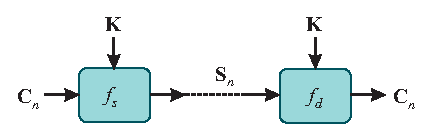
\includegraphics[width=0.75\columnwidth]{Slike/vektorska_slika_2.eps}
    \caption{\label{oblika_signalov_2} Primer vektorske slike EPS.}
\end{figure}

Za vključevanje bitnih slik je v predlogi na voljo makro \textbackslash jpgslika. Prvi parameter v makroju \textbackslash jpgslika je podnaslov, drugi pa je ime datoteke s sliko (privzeta končnica je .jpg) in hkrati tudi oznaka za sklicevanje na sliko. Pri uporabi tega ukaza morajo biti slikovne datoteke v korenu delovnega direktorija. Slike so v tekst vključene v originalni velikosti.

Slika \ref{bitna_slika} predstavlja primer vključitve bitne slike JPG formata velikosti 9,4 x 7,6 cm.

\begin{figure}[h]
    \centering
    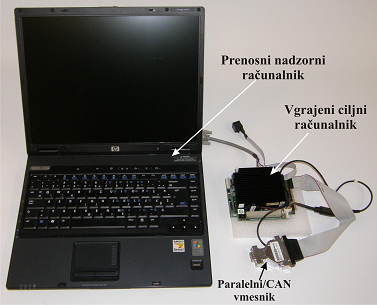
\includegraphics[width=9.4cm, height=7.6cm]{Slike/bitna_slika.png}
    \caption{\label{bitna_slika} Primer vključitve bitne slike: sistem vodenja.}
\end{figure}

\chapter{Namestitev programskih orodij za urejanje LaTeX dokumentov} \label{prilogaC}

\section{Sistemi Windows}

\begin{description}
    \item[Korak 1] Namestitev paketa MiKTeX, ki je prevajalnik za dokumente, napisane v okolju LaTeX. Datoteke so dostopne na spletu: \url{http://miktex.org/}
    \item[Korak 2] Namestitev tekstovnega urejevalnika. Nekaj priporočenih:
    \begin{itemize}[noitemsep]
        \item TeXstudio (\url{http://texstudio.sourceforge.net/})
        \item Texmaker (\url{http://www.xm1math.net/texmaker/})
        \item Geany (\url{http://www.geany.org/})
        \item WinEdt (\url{http://www.winedt.com/})
    \end{itemize}
    \item[Korak 3] Namestitev ogledovalnika PostScript dokumentov:
    \begin{itemize}[noitemsep]
        \item modul GhostScript
        \item modul GhostView
    \end{itemize}
    Datoteke so dostopne na: \url{www.cs.wisc.edu/~ghost/}
\end{description}

Pri prvem prevajanju se lahko zgodi, da MiKTeX poskusi namestiti potrebne LaTeX knjižnice (pakete), kar mu je treba dovoliti, sicer predloga ne more delovati. Zaradi prenašanja in nameščanja prvo prevajanje lahko spodleti, kar je napaka paketa MiKTeX.

\section{Sistemi Linux}

Na sistemih Linux je potrebno za uporabo predloge namestiti naslednje pakete:

\begin{itemize}[noitemsep]
    \item \texttt{texlive-lang-european}
    \item \texttt{texlive-lang-greek}
    \item \texttt{texlive-latex-extra}
\end{itemize}

Imena paketov so povzeta po znani Linux distribuciji Ubuntu. V drugih distribucijah se enaki paketi lahko imenujejo tudi malo drugače. Za urejanje dokumentov se priporočajo naslednji tekstovni urejevalniki:

\begin{itemize}[noitemsep]
    \item TeXstudio (paket \texttt{texstudio})
    \item Texmaker (paket \texttt{texmaker})
    \item Geany (paket \texttt{geany})
\end{itemize}

\end{document}
%%%%%%%%%%%%%%%%%%%%%%%%%%%%%%%%%%%%%%%%%%%%%%%%%%%%%%%%%%%%%%%%%%%%%%%%%%%%%%%%%%%%%%%%%%%%%%%%%%%%%%%%%%%%%%%%%%%%%%%%
